\documentclass[aspectratio=169, table]{beamer}

\usepackage[utf8]{inputenc}
\usepackage{listings} 

\usetheme{Pradita}

\subtitle{IF140303-Web Application Development}

\title{Session-07:\\
\Huge{
Phoenix Framework \& PostgreSQL\\
\vspace{-20pt}
}
}
\date[Serial]{\scriptsize{PRU/SPMI/FR-BM-18/0222}}
\author[Pradita]{\small{\textbf{Alfa Yohannis}}}

\lstdefinelanguage{Elixir} {
	keywords={case, def, defmodule, do, end, for, if, else, true, false},
	basicstyle=\ttfamily\small,
	keywordstyle=\color{blue}\bfseries,
	ndkeywords={@moduledoc, iex, Enum, @doc},
	ndkeywordstyle=\color{purple}\bfseries,
	sensitive=true,
	numbers=left,
	numberstyle=\tiny\color{gray},
	breaklines=true,
	frame=lines,
	backgroundcolor=\color{lightgray!10},
	tabsize=2,
	comment=[l]{\#},
	morecomment=[s]{/*}{*/},
	commentstyle=\color{gray}\ttfamily,
	showstringspaces=false,
	% string settings
	morestring=[b]",
	morestring=[b]',
	stringstyle=\color{black}\ttfamily, % default, will be overridden
	moredelim=[s][\color{blue}\ttfamily]{"}{"},   % double quotes
	moredelim=[s][\color{teal}\ttfamily]{'}{'}    % single quotes
}


\lstdefinelanguage{bash} {
	keywords={},
	basicstyle=\ttfamily\small,
	keywordstyle=\color{blue}\bfseries,
	ndkeywords={iex},
	ndkeywordstyle=\color{purple}\bfseries,
	sensitive=true,
	commentstyle=\color{gray},
	stringstyle=\color{red},
	numbers=left,
	numberstyle=\tiny\color{gray},
	breaklines=true,
	frame=lines,
	backgroundcolor=\color{lightgray!10},
	tabsize=2,
	comment=[l]{\#},
	morecomment=[s]{/*}{*/},
	commentstyle=\color{gray}\ttfamily,
	stringstyle=\color{purple}\ttfamily,
	showstringspaces=false
}

\begin{document}
	
	\frame{\titlepage}
	
		\begin{frame}[fragile]
		\frametitle{Contents}
		\vspace{20pt}
		\begin{columns}[t]
			\column{0.5\textwidth}
			\tableofcontents[sections={1-6}]
			
			\column{0.5\textwidth}
			\tableofcontents[sections={7-99}]
		\end{columns}
	\end{frame}


\section{Introduction to Phoenix Framework}

\begin{frame}[fragile]{Phoenix in a Nutshell}
\vspace{20pt}
Phoenix is a full-stack Elixir web framework for scalable, real-time apps. Built on the Erlang VM (BEAM), it uses lightweight processes for massive concurrency and fault tolerance. It follows MVC, separating data, logic, and presentation.

\begin{itemize}
  \item Fast request/response; real-time via Channels/WebSockets.
  \item Ecto for database access and composable queries.
  \item HEEx templates for safe, component-friendly HTML.
\end{itemize}

Ideal for chats, interactive dashboards, online games, and high-availability services of any size.
\end{frame}

\section{Understanding the MVC Pattern in Phoenix}

\begin{frame}[fragile]{MVC Pattern in Phoenix}
\vspace*{20pt}

\begin{figure}[h]
  \centering
  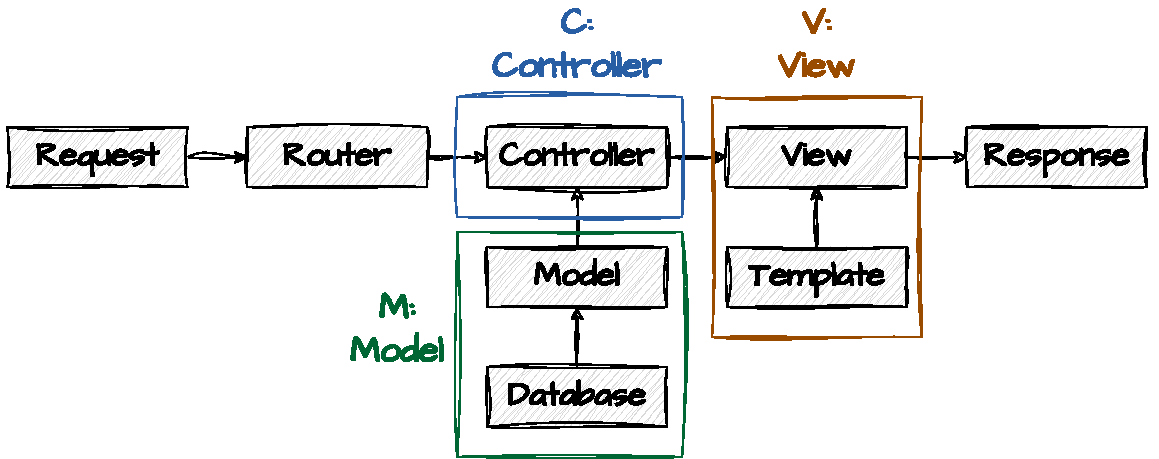
\includegraphics[width=.8\textwidth]{../../assets/phoenix-mvc.pdf}
\end{figure}

Phoenix uses the Model-View-Controller (MVC) pattern for clear, reusable, and maintainable structure.  
\textbf{Model} handles data and logic via Ecto.  
\textbf{View} renders templates using HEEx.  
\textbf{Controller} manages requests and responses.

\end{frame}


\begin{frame}[fragile]{Request in Phoenix}
\vspace*{20pt}

\begin{columns}
  \begin{column}[T]{0.52\textwidth}
    A request in Phoenix starts when a client (such as a web browser)  
    sends an HTTP request to the server. The router matches this request  
    to the appropriate controller and action for processing.

    \begin{itemize}
      \item The request contains a path, method, headers, and parameters.
      \item The controller receives the request via the \texttt{conn} struct.
      \item Phoenix passes the processed result to the view for rendering.
    \end{itemize}
  \end{column}

  \begin{column}[T]{0.43\textwidth}
\begin{lstlisting}[language=bash]
GET /about HTTP/1.1
Host: localhost:4000
User-Agent: Mozilla/5.0
Accept: text/html
\end{lstlisting}

This HTTP request is routed to  
\texttt{PageController.about/2},  
which prepares data for rendering.
  \end{column}
\end{columns}
\end{frame}


\begin{frame}[fragile]{Router in Phoenix}
\vspace{20pt}

The router maps incoming HTTP requests to the appropriate controller and action.  
In Phoenix, routes are defined in the \texttt{router.ex} file. It checks the request path and method (GET, POST, etc.) to decide which controller and function should handle it.

\begin{lstlisting}[language=Elixir]
scope "/", HelloWeb do
  pipe_through :browser

  get "/", PageController, :home
  get "/about", PageController, :about
  get "/queue/new", QueueController, :new
end
\end{lstlisting}

This example maps GET requests like \texttt{/about} and \texttt{/queue/new} to their respective controller actions.
\end{frame}

\begin{frame}[fragile]{Controller in Phoenix}
\vspace{15pt}

\begin{columns}
  \begin{column}[t]{0.45\textwidth}
    \begin{itemize}
      \item Controllers act as a bridge between models (data) and views (presentation).
      \item They process incoming requests and may interact with the database.
      \item Each action corresponds to a function handling a specific request.
      \item Uses \texttt{render/3} to return the proper HTML template.
      \item The \texttt{conn} argument holds request and response data.
    \end{itemize}
  \end{column}

  \begin{column}[t]{0.5\textwidth}
\begin{lstlisting}[language=Elixir]
defmodule HelloWeb.PageController do
  use HelloWeb, :controller

  def about(conn, _params) do
    render(conn, :about, layout: false)
  end

  def home(conn, _params) do
    render(conn, :home, layout: false)
  end
end
\end{lstlisting}
  \end{column}
\end{columns}
\end{frame}

\begin{frame}[fragile]{Model and Database Interaction}
\vspace*{20pt}

\begin{columns}
  \begin{column}[T]{0.52\textwidth}
    Models represent and manage application data stored in a database.  
    Phoenix uses \texttt{Ecto}, a robust database wrapper and query generator, for data operations.

    \begin{itemize}
      \item Defines schemas mapping Elixir structs to database tables.
      \item Supports CRUD operations (Create, Read, Update, Delete).
      \item Ensures data validation and integrity through changesets.
    \end{itemize}
  \end{column}
 
  \begin{column}[T]{0.43\textwidth}
\begin{lstlisting}[language=Elixir]
defmodule Hello.Accounts.User do
  use Ecto.Schema

  schema "users" do
    field :name, :string
    field :email, :string
    field :age, :integer

    timestamps()
  end
end
\end{lstlisting}
  \end{column}
\end{columns}
\end{frame}

\begin{frame}[fragile]{View and Template in Phoenix}
\vspace*{20pt}

\begin{columns}
  \begin{column}[T]{0.6\textwidth}
    Views are responsible for rendering responses such as HTML or JSON.  
    They receive data from controllers and apply templates to generate the final output.

    \begin{itemize}
      \item Use \texttt{HEEx} (HTML Embedded Elixir) for dynamic HTML rendering.
      \item Contain no business logic — only presentation logic.
      \item Render controller data into client-ready formats.
    \end{itemize}
  \end{column}

  \begin{column}[T]{0.35\textwidth}

\begin{lstlisting}[language=bash]
<h1>
	<b>
		Hello World!
	</b>
</h1>
\end{lstlisting}

A simple HEEx template example  
for the \texttt{about} page.
  \end{column}
\end{columns}
\end{frame}

\begin{frame}[fragile]{Response in Phoenix}
\vspace*{20pt}

\begin{columns}
  \begin{column}[T]{0.52\textwidth}
    After the view processes data and applies the template,  
    Phoenix generates a final response and sends it back to the client.

    \begin{itemize}
      \item Responses can be HTML, JSON, or other content types.
      \item Determined by the request and controller action.
      \item The client (e.g., browser) renders the returned content.
    \end{itemize}
  \end{column}

  \begin{column}[T]{0.43\textwidth}
\begin{lstlisting}[language=bash]
GET /about
--> Returns:
about.html.heex

<h1><b>Hello World!</b></h1>
\end{lstlisting}

Example of an HTML response  
for the \texttt{/about} page.
  \end{column}
\end{columns}
\end{frame}

\subsection{Integrating All Components}

\begin{frame}[fragile]{Integrating All Components}
\vspace{20pt}

To summarize the MVC flow in Phoenix:

\begin{enumerate}
  \item \texttt{Router} receives the HTTP request and forwards it to the appropriate \texttt{Controller}.
  \item \texttt{Controller} handles business logic and may interact with the \texttt{Model} to fetch or update data.
  \item \texttt{View} takes data from the \texttt{Controller} and uses a \texttt{Template} to render the response.
  \item \texttt{Response} is sent back to the client, completing the request/response cycle.
\end{enumerate}

By dividing the application into these components, Phoenix ensures each part has a single responsibility, improving maintainability and scalability over time.
\end{frame}


\section{Installing PostgreSQL}

\begin{frame}[fragile]{Installing PostgreSQL (Part 1)}
\vspace{20pt}

PostgreSQL is a powerful open-source object-relational database system.  
It will serve as the database for our Phoenix web application.  
Follow these steps to install PostgreSQL:

\begin{enumerate}
  \item Update package list:
  \begin{lstlisting}[language=bash]
  sudo apt update
  \end{lstlisting}

  \item Install PostgreSQL and remove old configurations:
  \begin{lstlisting}[language=bash]
  sudo apt install postgresql -y --purge
  \end{lstlisting}

  \item Enable and start the PostgreSQL service:
  \begin{lstlisting}[language=bash]
  sudo systemctl enable postgresql
  sudo systemctl start postgresql
  sudo systemctl status postgresql
  \end{lstlisting}
\end{enumerate}
\end{frame}

\begin{frame}[fragile]{Installing PostgreSQL (Part 2)}
\vspace{20pt}

\begin{enumerate}
  \setcounter{enumi}{3}
  \item (Optional) Install pgAdmin4 for graphical management:
  \begin{lstlisting}[language=bash]
  sudo apt install pgadmin4-desktop -y --purge
  \end{lstlisting}

  \item Switch to the PostgreSQL user:
  \begin{lstlisting}[language=bash]
  sudo -i -u postgres
  \end{lstlisting}

  \item Set a password for the \texttt{postgres} user (for development, e.g. \texttt{1234}):
  \begin{lstlisting}[language=bash]
  psql> \password postgres
  \end{lstlisting}
\end{enumerate}

After setup, PostgreSQL is ready for use with Phoenix.
\end{frame}


\section{Installing Phoenix Framework}

\begin{frame}[fragile]{Installing Phoenix Framework (Part 1)}
\vspace{20pt}

\begin{columns}
  \begin{column}[T]{0.5\textwidth}
    Phoenix Framework, built on Elixir, enables scalable, real-time web development.  
    Follow these steps to install Phoenix and set up a new project:

    \begin{enumerate}
      \item Install \texttt{inotify-tools} to detect file changes.
      \begin{lstlisting}[language=bash]
sudo apt install inotify-tools
      \end{lstlisting}

      \item Check Elixir version.
      \begin{lstlisting}[language=bash]
elixir -v
      \end{lstlisting}
    \end{enumerate}
  \end{column}

  \begin{column}[T]{0.5\textwidth}
    \begin{enumerate}
      \setcounter{enumi}{2}
		      \item Install Hex, the package manager for Elixir.
      \begin{lstlisting}[language=bash]
mix local.hex
      \end{lstlisting}
      \item Install the Phoenix project generator.
      \begin{lstlisting}[language=bash]
mix archive.install hex phx_new
      \end{lstlisting}

      \item Create a new project named \texttt{hello}.
      \begin{lstlisting}[language=bash]
mix phx.new hello
      \end{lstlisting}

     
    \end{enumerate}
  \end{column}
\end{columns}
\end{frame}

\begin{frame}[fragile]{Installing Phoenix Framework (Part 2)}
\vspace{20pt}

\begin{columns}
  \begin{column}[T]{0.6\textwidth}
    \begin{enumerate}
	   \item Enter the project directory and open in VS Code.
      \begin{lstlisting}[language=bash]
cd hello
code .
      \end{lstlisting}
      \item Edit database settings in \texttt{config/dev.exs}  
      and \texttt{config/test.exs}, set password to \texttt{1234}.
      
      \item Fetch dependencies and create the database.
      \begin{lstlisting}[language=bash]
mix deps.get
mix ecto.create
      \end{lstlisting}
    \end{enumerate}
  \end{column}

  \begin{column}[T]{0.4\textwidth}
    \begin{enumerate}
      \setcounter{enumi}{2}
      \item Start the Phoenix server.
      \begin{lstlisting}[language=bash]
mix phx.server
iex -S mix phx.server
      \end{lstlisting}

      \item Visit the app in your browser:
      \begin{lstlisting}[language=bash]
http://localhost:4000
      \end{lstlisting}

      Phoenix is now installed and running!
    \end{enumerate}
  \end{column}
\end{columns}
\end{frame}

\section{Routing in Phoenix}

\begin{frame}[fragile]{Routing in Phoenix}
\vspace{15pt}

Routing in Phoenix defines how incoming requests are mapped to specific controllers and actions.  
Follow these steps to configure routes in your application:

\begin{columns}
  \begin{column}[T]{0.55\textwidth}
    \begin{enumerate}
      \item Open \texttt{lib/hello\_web/router.ex} and define the following routes:
\begin{lstlisting}[language=Elixir, basicstyle=\ttfamily\footnotesize]
scope "/", HelloWeb do
  pipe_through :browser
  
  get "/", PageController, :home
  get "/about", PageController, :about
  get "/queue/new", QueueController, :new
end
\end{lstlisting}
    \end{enumerate}
  \end{column}

  \begin{column}[T]{0.45\textwidth}
    \begin{enumerate}
        \item \texttt{pipe\_through :browser}: Applies the default browser stack, including sessions, cookies, and request handling.
        \item \texttt{get "/"}: Maps the root URL to the \texttt{home} action in \texttt{PageController}.
        \item Similarly, \texttt{get "/about"} and \texttt{get "/queue/new"} define routes for the About page and New Queue page.
    \end{enumerate}
  \end{column}
\end{columns}
\end{frame}

\section{Creating Page and Queue Controllers}

\begin{frame}[fragile]{Creating Controllers (Part 1)}
\vspace{20pt}

\begin{columns}
  \begin{column}[T]{0.5\textwidth}
    Controllers in Phoenix handle logic and rendering for different web pages.  
    Let’s define two controllers: one for general pages and another for queue actions.

    \begin{enumerate}
      \item Define \texttt{PageController} to handle the home and about pages.
      \item \texttt{use HelloWeb, :controller}: Imports Phoenix controller functionality.
      \item \texttt{about/2}: Renders \texttt{about.html.heex} without layout.
      \item \texttt{home/2}: Renders \texttt{home.html.heex}.
    \end{enumerate}
  \end{column}

  \begin{column}[T]{0.47\textwidth}
\begin{lstlisting}[language=Elixir, basicstyle=\ttfamily\footnotesize]
defmodule HelloWeb.PageController do
  use HelloWeb, :controller

  def about(conn, _params) do
    render(conn, :about, layout: false)
  end

  def home(conn, _params) do
    render(conn, :home, layout: false)
  end
end
\end{lstlisting}
  \end{column}
\end{columns}
\end{frame}


\begin{frame}[fragile]{Creating Controllers (Part 2)}
\vspace{20pt}

\begin{enumerate}
  \setcounter{enumi}{2}
  \item Define \texttt{QueueController} to handle the new queue page:
\begin{lstlisting}[language=Elixir, basicstyle=\ttfamily\footnotesize]
defmodule HelloWeb.QueueController do
  use HelloWeb, :controller

  def new(conn, _params) do
    render(conn, :new, layout: false)
  end
end
\end{lstlisting}

  \item \texttt{new/2}: Renders \texttt{new.html.heex} for the queue creation page.
\end{enumerate}
\end{frame}


\section{Rendering HTML Pages}

\begin{frame}[fragile]{Rendering HTML Templates in Phoenix}
\vspace{20pt}

\begin{columns}
  \begin{column}[T]{0.52\textwidth}
    HTML templates define the structure of web pages rendered by controllers.  
    Let’s create two templates — one for the About page and one for the New Queue page.

    \textbf{About Template:}
\begin{lstlisting}[language=bash, basicstyle=\ttfamily\footnotesize]
<h1>
	<b>
		Hello World!
	</b>
</h1>
\end{lstlisting}
    This simple HTML template displays a “Hello World” message for the About page.
  \end{column}

  \begin{column}[T]{0.43\textwidth}
    \textbf{New Queue Template:}
\begin{lstlisting}[language=bash, basicstyle=\ttfamily\footnotesize]
<h1>
	<b>
		This is the New Queue Page
	</b>
</h1>
\end{lstlisting}

    This template displays a simple heading for the New Queue page.  
    Templates like these are rendered through controller actions using \texttt{render/3}.
  \end{column}
\end{columns}
\end{frame}


\section{Embedding Templates}

\begin{frame}[fragile]{Embedding Templates in Phoenix}
\vspace{20pt}

\begin{columns}
  \begin{column}[T]{0.5\textwidth}
\begin{lstlisting}[language=Elixir, basicstyle=\ttfamily\footnotesize]
defmodule HelloWeb.QueueHTML do
  @moduledoc """
  This module contains the pages rendered
  by the QueueController.

  See the `queue_html` directory for all
  available templates.
  """
  use HelloWeb, :html

  embed_templates "queue_html/*"
end
\end{lstlisting}
  \end{column}

  \begin{column}[T]{0.45\textwidth}
    Phoenix allows you to embed HTML templates directly inside modules,  
    making it easier to manage multiple templates for a single controller.  
    In this example, the \texttt{QueueHTML} module is used for  
    \texttt{QueueController} templates.

    \begin{itemize}
      \item The \texttt{embed\_templates} macro automatically imports  
      all templates from the \texttt{queue\_html} directory.
      \item This approach keeps controllers lightweight and  
      simplifies the rendering workflow.
    \end{itemize}
  \end{column}
\end{columns}
\end{frame}


\section{Summary}
\begin{frame}[fragile]{Summary}
\vspace{20pt}

\begin{itemize}
  \item \textbf{PostgreSQL:} Installed and configured as the database for Phoenix apps.
  \item \textbf{Phoenix Setup:} Installed dependencies, created a new project, and ran the server.
  \item \textbf{MVC Pattern:} Organized the app with \texttt{Model}, \texttt{View}, and \texttt{Controller}.
  \item \textbf{Routing:} Mapped HTTP requests to controller actions.
  \item \textbf{Controllers:} Built \texttt{PageController} and \texttt{QueueController}.
  \item \textbf{Templates:} Rendered HTML views using HEEx templates.
  \item \textbf{Embedded Templates:} Used \texttt{embed\_templates} for easy template management.
  \item \textbf{Result:} A working Phoenix web app connected to PostgreSQL.
\end{itemize}
\end{frame}


\end{document}
